\documentclass[tikz]{standalone}
\usepackage{fourier}
\usepackage{tikz}

\begin{document}
	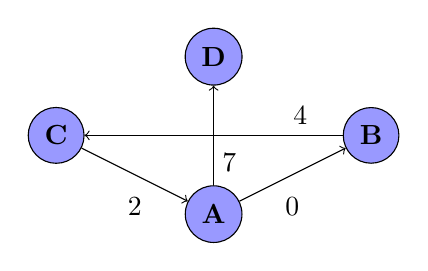
\begin{tikzpicture}
		\node[draw,circle,fill=blue!40!white](a) at (0,1) {\textbf{A}};
		\node[draw,circle,fill=blue!40!white](b) at (2,2) {\textbf{B}};
		\node[draw,circle,fill=blue!40!white](c) at (-2,2) {\textbf{C}};
		\node[draw,circle,fill=blue!40!white](d) at (0,3) {\textbf{D}};
		\node[draw=none] at (1,1.1) {$0$};
		\node[draw=none] at (-1,1.1) {$2$};
		\node[draw=none] at (1.1,2.25) {$4$};
		\node[draw=none] at (0.2,1.65) {$7$};
		\draw[->] (a)--(b);
		\draw[->] (b)--(c);
		\draw[->] (c)--(a);
		\draw[->] (a)--(d);
	\end{tikzpicture}
\end{document}
